
\documentclass[10pt, a4paper]{article}

\usepackage[margin=0.75in]{geometry}
\usepackage{amsmath, amssymb, amsthm, mathtools}
\usepackage{enumitem}
\usepackage[T1]{fontenc}
\usepackage{lmodern}
\usepackage{microtype}
\usepackage{hyperref}
\usepackage{xcolor}

\usepackage{graphicx}                % \includegraphics
\usepackage{float}                   % [H] placement
\usepackage{caption}                 % better captions
\usepackage{subcaption}              % subfigures side by side
\usepackage{tikz}                    % drawing
\usepackage{pgfplots}                % function plots
\pgfplotsset{compat=1.18}

\usepackage{booktabs}                % \toprule, \midrule, \bottomrule
\usepackage{tabularx}                % auto-width columns (X type)
\usepackage{longtable}               % multi-page tables

% \usepackage{listings}
% \lstset{
%   basicstyle=\ttfamily\small,
%   keywordstyle=\color{blue}\bfseries,
%   commentstyle=\color{gray},
%   stringstyle=\color{red!70!black},
%   numbers=left, numberstyle=\tiny\color{gray},
%   frame=single, breaklines=true,
%   tabsize=2
% }
% \usepackage{algorithm}
% \usepackage{algpseudocode}


\newcommand{\note}[1]{\par{\small\textit{#1}}\par}

\usetikzlibrary{
  arrows.meta,          % modern arrow tips
  positioning,          % relative node placement (right=of, above=of)
  calc,                 % coordinate math
  shapes.geometric,     % triangles, diamonds, etc.
  shapes.misc,          % crosses, rounded rectangles
  decorations.pathmorphing, % zigzag, snake lines
  decorations.markings, % marks along paths
  patterns,             % hatching, dots fills
  automata,             % state machines (CS courses)
  trees,                % tree diagrams
  fit,                  % grouping nodes
  backgrounds,          % background layers
  matrix,               % matrix of nodes
}

\usepackage[most,skins,breakable]{tcolorbox}
\usepackage{titlesec}
\usepackage{fancyhdr}

\hypersetup{colorlinks=true, linkcolor=blue!60!black, urlcolor=blue!70!black}
\setlength{\parindent}{0pt}
\setlength{\parskip}{3pt}
\setlist{nosep, leftmargin=1.5em}

\pagestyle{fancy}
\fancyhf{}
\lhead{{\small MATH 999 \quad Chapter 1: Foundations of Widget Theory}}
\rhead{{\small Fall 2099}}
\cfoot{\thepage}

\titleformat{\section}{\Large\bfseries}{\thesection}{6pt}{}
\titleformat{\subsection}{\large\bfseries}{\thesubsection}{4pt}{}

\newtheorem{theorem}{Theorem}[section]
\newtheorem{lemma}[theorem]{Lemma}
\newtheorem{proposition}[theorem]{Proposition}
\newtheorem{corollary}[theorem]{Corollary}
\theoremstyle{definition}
\newtheorem{definition}[theorem]{Definition}
\newtheorem{example}[theorem]{Example}
\theoremstyle{remark}
\newtheorem{remark}[theorem]{Remark}


\definecolor{defblue}{HTML}{1B4F72}
\definecolor{defbluebg}{HTML}{D6EAF8}
\definecolor{thmred}{HTML}{922B21}
\definecolor{thmredbg}{HTML}{FADBD8}
\definecolor{exgreen}{HTML}{1E8449}
\definecolor{exgreenbg}{HTML}{D5F5E3}
\definecolor{whyorange}{HTML}{B9770E}
\definecolor{whyorangebg}{HTML}{FDEBD0}
\definecolor{sumpurple}{HTML}{6C3483}
\definecolor{sumpurplebg}{HTML}{E8DAEF}
\definecolor{codegray}{HTML}{2C3E50}
\definecolor{codegraybg}{HTML}{EAECEE}
\definecolor{algoteal}{HTML}{117A65}
\definecolor{algotealbg}{HTML}{D1F2EB}
\definecolor{noteyellow}{HTML}{F9E79F}

\newtcolorbox{defbox}[1][]{%
  enhanced jigsaw, breakable,
  colback=defbluebg, colframe=defblue, coltitle=white,
  fonttitle=\bfseries, title={#1},
  arc=1.5mm, boxrule=0.8pt,
  left=6pt, right=6pt, top=4pt, bottom=4pt,
  pad at break*=2mm,
  drop shadow southeast}
\newtcolorbox{thmbox}[1][]{%
  enhanced jigsaw, breakable,
  colback=thmredbg, colframe=thmred, coltitle=white,
  fonttitle=\bfseries, title={#1},
  arc=1.5mm, boxrule=0.8pt,
  left=6pt, right=6pt, top=4pt, bottom=4pt,
  pad at break*=2mm,
  drop shadow southeast}
\newtcolorbox{exbox}[1][]{%
  enhanced jigsaw, breakable,
  colback=exgreenbg, colframe=exgreen, coltitle=white,
  fonttitle=\bfseries, title={#1},
  arc=1.5mm, boxrule=0.8pt,
  left=6pt, right=6pt, top=4pt, bottom=4pt,
  pad at break*=2mm,
  drop shadow southeast}
\newtcolorbox{whybox}[1][]{%
  enhanced jigsaw, breakable,
  colback=whyorangebg, colframe=whyorange, coltitle=white,
  fonttitle=\bfseries, title={#1},
  arc=1.5mm, boxrule=0.8pt,
  left=6pt, right=6pt, top=4pt, bottom=4pt,
  pad at break*=2mm,
  drop shadow southeast}
\newtcolorbox{sumbox}[1][]{%
  enhanced jigsaw, breakable,
  colback=sumpurplebg, colframe=sumpurple, coltitle=white,
  fonttitle=\bfseries, title={#1},
  arc=1.5mm, boxrule=0.8pt,
  left=6pt, right=6pt, top=4pt, bottom=4pt,
  pad at break*=2mm,
  drop shadow southeast}
\newtcolorbox{codebox}[1][]{%
  enhanced jigsaw, breakable,
  colback=codegraybg, colframe=codegray, coltitle=white,
  fonttitle=\bfseries, title={#1},
  arc=1.5mm, boxrule=0.8pt,
  left=6pt, right=6pt, top=4pt, bottom=4pt,
  pad at break*=2mm,
  drop shadow southeast}
\newtcolorbox{algobox}[1][]{%
  enhanced jigsaw, breakable,
  colback=algotealbg, colframe=algoteal, coltitle=white,
  fonttitle=\bfseries, title={#1},
  arc=1.5mm, boxrule=0.8pt,
  left=6pt, right=6pt, top=4pt, bottom=4pt,
  pad at break*=2mm,
  drop shadow southeast}

\newcommand{\R}{\mathbb{R}}
\newcommand{\N}{\mathbb{N}}
\newcommand{\Q}{\mathbb{Q}}
\newcommand{\Z}{\mathbb{Z}}
\newcommand{\C}{\mathbb{C}}
\newcommand{\eps}{\varepsilon}

\title{\textbf{MATH 999: Introduction to Widget Theory}\\[4pt]
  {\Large Chapter 1: Foundations of Widget Theory}}
\author{{\small Exemplar University \quad Fall 2099 \quad Prof.\ A.\ Placeholder}}
\date{}

\begin{document}
\maketitle
\thispagestyle{fancy}
\tableofcontents
\newpage

% ═══════════════════════════════════════════════════════════════════════
% EXAMPLE CONTENT: shows every element the agent can use.
% ═══════════════════════════════════════════════════════════════════════

\section{Basic Definitions}

We need a way to measure the size of a widget that captures both its
width and depth.

\begin{defbox}[Definition: Widget Norm]
Let $W$ be a widget space. For $w \in W$, the \textbf{widget norm} is
\[
  \|w\|_W = \sup_{k \ge 1} |w_k| \cdot 2^{-k}.
\]
We say $w$ is \textbf{finite} if $\|w\|_W < \infty$.
\end{defbox}

The factor $2^{-k}$ ensures later components contribute less.

\begin{exbox}[Example: Computing the widget norm]
Let $w = (3, 1, 4, 1, 5, 9, \ldots)$ where $w_k$ is the $k$-th digit of $\pi$.
\note{The sup is attained at $k=1$ because the exponential decay $2^{-k}$ dominates for all later terms.}
\begin{align*}
  \|w\|_W &= \sup\!\left\{\frac{3}{2},\; \frac{1}{4},\; \frac{4}{8},\;
             \frac{1}{16},\; \frac{5}{32},\; \ldots\right\}
          = \frac{3}{2}.
\end{align*}
\end{exbox}


Here is a plot of the decay $2^{-k}$ showing why later components
are negligible:

\begin{center}
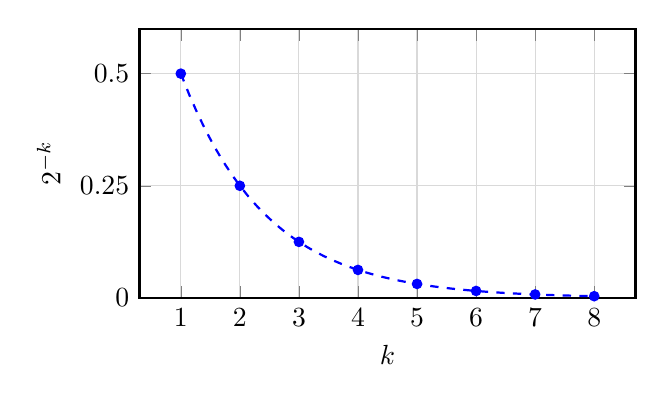
\begin{tikzpicture}
  \begin{axis}[
    width=0.65\textwidth, height=5cm,
    xlabel={$k$}, ylabel={$2^{-k}$},
    xtick={1,2,...,8}, ytick={0,0.25,0.5},
    ymin=0, ymax=0.6,
    grid=major, grid style={gray!30},
    thick
  ]
  \addplot[blue, mark=*, mark size=1.5pt, only marks]
    coordinates {(1,0.5)(2,0.25)(3,0.125)(4,0.0625)
                 (5,0.03125)(6,0.015625)(7,0.0078)(8,0.0039)};
  \addplot[blue, dashed, domain=1:8, samples=50]{2^(-x)};
  \end{axis}
\end{tikzpicture}
\end{center}


\begin{figure}[H]
  \centering
  \begin{subfigure}[t]{0.48\textwidth}
    \centering
    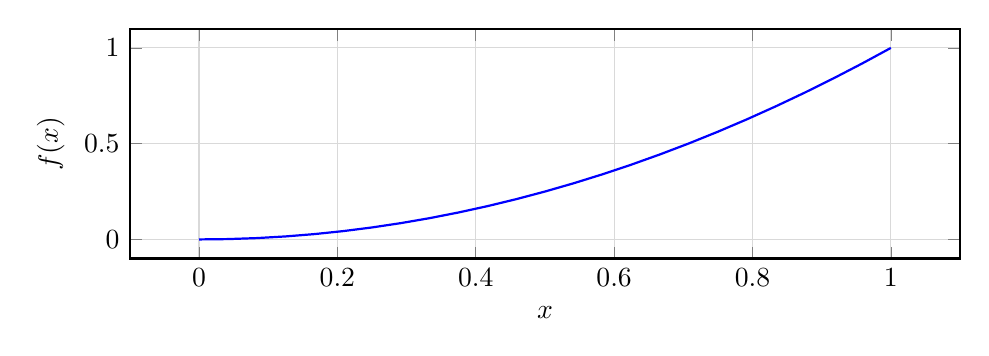
\begin{tikzpicture}
      \begin{axis}[
        width=\textwidth, height=4.5cm,
        xlabel={$x$}, ylabel={$f(x)$},
        domain=0:1, thick, grid=major, grid style={gray!30}
      ]
      \addplot[blue]{x^2};
      \end{axis}
    \end{tikzpicture}
    \caption{$f(x) = x^2$}
  \end{subfigure}\hfill
  \begin{subfigure}[t]{0.48\textwidth}
    \centering
    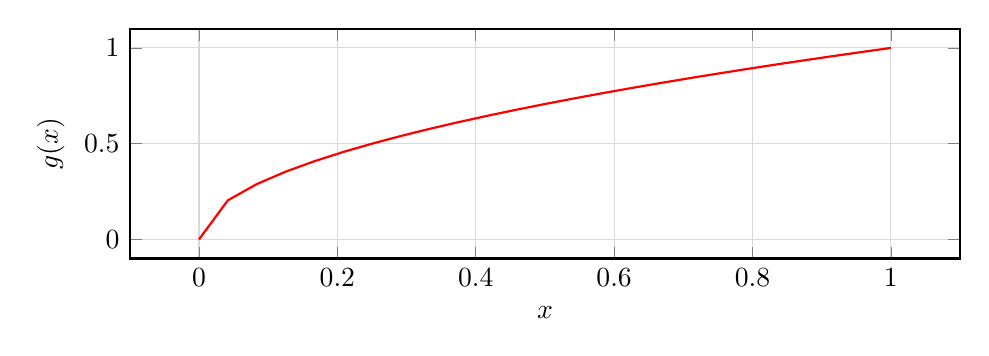
\begin{tikzpicture}
      \begin{axis}[
        width=\textwidth, height=4.5cm,
        xlabel={$x$}, ylabel={$g(x)$},
        domain=0:1, thick, grid=major, grid style={gray!30}
      ]
      \addplot[red]{sqrt(x)};
      \end{axis}
    \end{tikzpicture}
    \caption{$g(x) = \sqrt{x}$}
  \end{subfigure}
  \caption{Two functions on $[0,1]$: $x^2$ is convex, $\sqrt{x}$ is concave.}
  \label{fig:two-functions}
\end{figure}


\begin{sumbox}[Section Summary]
\begin{itemize}
  \item The widget norm $\|w\|_W = \sup_k |w_k| \cdot 2^{-k}$ measures size with exponential decay.
  \item $\|w\|_W = 0$ iff $w = 0$. The norm satisfies the triangle inequality.
  \item Later components contribute exponentially less, which is the key to all convergence arguments.
\end{itemize}
\end{sumbox}


\section{The Main Theorem}

Every bounded widget sequence has a convergent subsequence.

\begin{thmbox}[Theorem: Widget Approximation Theorem]
Let $(w^{(n)})$ be a sequence of widgets with $\|w^{(n)}\|_W \le M$ for
all $n$. Then there exists a subsequence $(w^{(n_j)})$ and a widget
$w^* \in W$ such that
$\|w^{(n_j)} - w^*\|_W \to 0$ as $j \to \infty$.
\end{thmbox}

\begin{proof}
We construct $w^*$ component by component using a diagonal argument.

\textbf{Step 1.}
$(w^{(n)}_1)$ is bounded by $2M$.
By Bolzano-Weierstrass, extract a subsequence with $w^{(n^1_j)}_1 \to w^*_1$.

\textbf{Step 2.}
From that subsequence, extract a further one with $w^{(n^2_j)}_2 \to w^*_2$.

\textbf{Step 3.}
Continue for all $k$. The diagonal subsequence $w^{(n^j_j)}$
converges in every component.

\textbf{Step 4.}
Let $\eps > 0$. Choose $K$ with $M \cdot 2^{-K} < \eps/2$.
For $j$ large enough:
\[
  \|w^{(n^j_j)} - w^*\|_W
  \le \max\!\left(\max_{k \le K} |w^{(n^j_j)}_k - w^*_k| \cdot 2^{-k},\;
       M \cdot 2^{-K}\right) < \eps.
\]

We showed that every bounded widget sequence has a norm-convergent
subsequence.
\end{proof}

\begin{whybox}[Intuition]
Two ideas: Bolzano-Weierstrass applied infinitely many times
(once per component) plus diagonal extraction, and the $2^{-k}$ decay
meaning we only need finitely many components to be close.
\end{whybox}


The diagonal argument can be visualized as a table where we select
entries along the diagonal:

\begin{center}
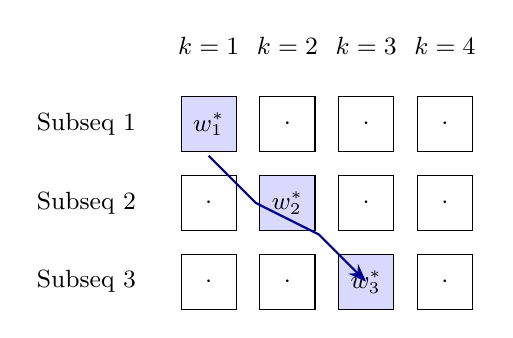
\begin{tikzpicture}[
  cell/.style={minimum size=7mm, draw, thin, font=\small},
  highlight/.style={cell, fill=blue!15, font=\small\bfseries},
]
  % Header row
  \node at (0.5, 3.5) {\small $k=1$};
  \node at (1.5, 3.5) {\small $k=2$};
  \node at (2.5, 3.5) {\small $k=3$};
  \node at (3.5, 3.5) {\small $k=4$};
  % Row labels
  \node[anchor=east] at (-0.3, 2.5) {\small Subseq 1};
  \node[anchor=east] at (-0.3, 1.5) {\small Subseq 2};
  \node[anchor=east] at (-0.3, 0.5) {\small Subseq 3};
  % Grid
  \node[highlight] at (0.5, 2.5) {$w^*_1$};
  \node[cell]      at (1.5, 2.5) {$\cdot$};
  \node[cell]      at (2.5, 2.5) {$\cdot$};
  \node[cell]      at (3.5, 2.5) {$\cdot$};
  \node[cell]      at (0.5, 1.5) {$\cdot$};
  \node[highlight] at (1.5, 1.5) {$w^*_2$};
  \node[cell]      at (2.5, 1.5) {$\cdot$};
  \node[cell]      at (3.5, 1.5) {$\cdot$};
  \node[cell]      at (0.5, 0.5) {$\cdot$};
  \node[cell]      at (1.5, 0.5) {$\cdot$};
  \node[highlight] at (2.5, 0.5) {$w^*_3$};
  \node[cell]      at (3.5, 0.5) {$\cdot$};
  % Diagonal arrow
  \draw[-{Stealth}, thick, blue!60!black]
    (0.5, 2.1) -- (1.1, 1.5) -- (1.9, 1.1) -- (2.5, 0.5);
\end{tikzpicture}
\end{center}


\section{A Useful Lemma}

\begin{thmbox}[Lemma: Tail Bound]
If $\|w\|_W \le M$, then for all $K \ge 1$:
$\sup_{k > K} |w_k| \cdot 2^{-k} \le M$.
\end{thmbox}

\begin{proof}
$\sup_{k > K} |w_k| \cdot 2^{-k}$ is the supremum over a subset of
$\{|w_k| \cdot 2^{-k} : k \ge 1\}$, so it is at most the full
supremum, which is $\|w\|_W \le M$.
\end{proof}

\begin{whybox}[Intuition]
The tail of a widget (components $k > K$) contributes at most $M$ to
the norm. For the diagonal argument, this means we can ignore the tail
once $K$ is large enough.
\end{whybox}


\section{Showcase: All Available Tools}

Every tool the agent can use, demonstrated below.

\subsection{Auto-width Table (tabularx)}

\begin{center}
\begin{tabularx}{\textwidth}{X c c}
\toprule
\textbf{Property} & \textbf{Widget Norm} & \textbf{Sup Norm} \\
\midrule
Decay weighting & Yes ($2^{-k}$) & No \\
Tail control & Automatic & Manual \\
Useful for & Widget spaces & Function spaces \\
\bottomrule
\end{tabularx}
\end{center}

\subsection{Code Listing (codebox)}

\begin{codebox}[Python: Computing the widget norm]
\begin{verbatim}
def widget_norm(w):
    """Compute ||w||_W = sup |w_k| * 2^(-k)."""
    return max(abs(w[k]) * 2**(-(k+1))
               for k in range(len(w)))

# Example
w = [3, 1, 4, 1, 5, 9]
print(widget_norm(w))  # 1.5
\end{verbatim}
\end{codebox}

\subsection{Algorithm (algobox)}

\begin{algobox}[Algorithm: Widget Approximation via Diagonal Extraction]
\textbf{Input:} Bounded sequence $(w^{(n)})$ with $\|w^{(n)}\|_W \le M$\\
\textbf{Output:} Convergent subsequence $(w^{(n_j)})$

\begin{enumerate}[nosep]
  \item Set $S_0 = \{1, 2, 3, \ldots\}$
  \item For $k = 1, 2, 3, \ldots$:
    \begin{enumerate}[nosep, label=(\alph*)]
      \item Extract $S_k \subseteq S_{k-1}$ such that $w^{(n)}_k \to w^*_k$ along $S_k$
    \end{enumerate}
  \item Set $n_j =$ the $j$-th element of $S_j$ \quad (diagonal selection)
  \item Return $(w^{(n_j)})$
\end{enumerate}
\end{algobox}

\subsection{Inline Note Demo}

The widget norm is the foundation of everything that follows.

\note{Controlling $\|w^{(n)} - w^*\|_W$ is the goal of every convergence argument in this chapter.}

Every convergence argument in this chapter reduces to bounding this norm.

\subsection{Long Table Demo (longtable)}

\begin{longtable}{c l l}
\toprule
$k$ & $|w_k| \cdot 2^{-k}$ & Running sup \\
\midrule
\endhead
1 & $3/2 = 1.500$ & $1.500$ \\
2 & $1/4 = 0.250$ & $1.500$ \\
3 & $4/8 = 0.500$ & $1.500$ \\
4 & $1/16 = 0.063$ & $1.500$ \\
5 & $5/32 = 0.156$ & $1.500$ \\
6 & $9/64 = 0.141$ & $1.500$ \\
\bottomrule
\caption{Step-by-step computation of $\|w\|_W$ for $w = (3,1,4,1,5,9,\ldots)$.}
\end{longtable}


\end{document}
